\documentclass[1p]{elsarticle_modified}
%\bibliographystyle{elsarticle-num}

%\usepackage[colorlinks]{hyperref}
%\usepackage{abbrmath_seonhwa} %\Abb, \Ascr, \Acal ,\Abf, \Afrak
\usepackage{amsfonts}
\usepackage{amssymb}
\usepackage{amsmath}
\usepackage{amsthm}
\usepackage{scalefnt}
\usepackage{amsbsy}
\usepackage{kotex}
\usepackage{caption}
\usepackage{subfig}
\usepackage{color}
\usepackage{graphicx}
\usepackage{xcolor} %% white, black, red, green, blue, cyan, magenta, yellow
\usepackage{float}
\usepackage{setspace}
\usepackage{hyperref}

\usepackage{tikz}
\usetikzlibrary{arrows}

\usepackage{multirow}
\usepackage{array} % fixed length table
\usepackage{hhline}

%%%%%%%%%%%%%%%%%%%%%
\makeatletter
\renewcommand*\env@matrix[1][\arraystretch]{%
	\edef\arraystretch{#1}%
	\hskip -\arraycolsep
	\let\@ifnextchar\new@ifnextchar
	\array{*\c@MaxMatrixCols c}}
\makeatother %https://tex.stackexchange.com/questions/14071/how-can-i-increase-the-line-spacing-in-a-matrix
%%%%%%%%%%%%%%%

\usepackage[normalem]{ulem}

\newcommand{\msout}[1]{\ifmmode\text{\sout{\ensuremath{#1}}}\else\sout{#1}\fi}
%SOURCE: \msout is \stkout macro in https://tex.stackexchange.com/questions/20609/strikeout-in-math-mode

\newcommand{\cancel}[1]{
	\ifmmode
	{\color{red}\msout{#1}}
	\else
	{\color{red}\sout{#1}}
	\fi
}

\newcommand{\add}[1]{
	{\color{blue}\uwave{#1}}
}

\newcommand{\replace}[2]{
	\ifmmode
	{\color{red}\msout{#1}}{\color{blue}\uwave{#2}}
	\else
	{\color{red}\sout{#1}}{\color{blue}\uwave{#2}}
	\fi
}

\newcommand{\Sol}{\mathcal{S}} %segment
\newcommand{\D}{D} %diagram
\newcommand{\A}{\mathcal{A}} %arc


%%%%%%%%%%%%%%%%%%%%%%%%%%%%%5 test

\def\sl{\operatorname{\textup{SL}}(2,\Cbb)}
\def\psl{\operatorname{\textup{PSL}}(2,\Cbb)}
\def\quan{\mkern 1mu \triangleright \mkern 1mu}

\theoremstyle{definition}
\newtheorem{thm}{Theorem}[section]
\newtheorem{prop}[thm]{Proposition}
\newtheorem{lem}[thm]{Lemma}
\newtheorem{ques}[thm]{Question}
\newtheorem{cor}[thm]{Corollary}
\newtheorem{defn}[thm]{Definition}
\newtheorem{exam}[thm]{Example}
\newtheorem{rmk}[thm]{Remark}
\newtheorem{alg}[thm]{Algorithm}

\newcommand{\I}{\sqrt{-1}}
\begin{document}

%\begin{frontmatter}
%
%\title{Boundary parabolic representations of knots up to 8 crossings}
%
%%% Group authors per affiliation:
%\author{Yunhi Cho} 
%\address{Department of Mathematics, University of Seoul, Seoul, Korea}
%\ead{yhcho@uos.ac.kr}
%
%
%\author{Seonhwa Kim} %\fnref{s_kim}}
%\address{Center for Geometry and Physics, Institute for Basic Science, Pohang, 37673, Korea}
%\ead{ryeona17@ibs.re.kr}
%
%\author{Hyuk Kim}
%\address{Department of Mathematical Sciences, Seoul National University, Seoul 08826, Korea}
%\ead{hyukkim@snu.ac.kr}
%
%\author{Seokbeom Yoon}
%\address{Department of Mathematical Sciences, Seoul National University, Seoul, 08826,  Korea}
%\ead{sbyoon15@snu.ac.kr}
%
%\begin{abstract}
%We find all boundary parabolic representation of knots up to 8 crossings.
%
%\end{abstract}
%\begin{keyword}
%    \MSC[2010] 57M25 
%\end{keyword}
%
%\end{frontmatter}

%\linenumbers
%\tableofcontents
%
\newcommand\colored[1]{\textcolor{white}{\rule[-0.35ex]{0.8em}{1.4ex}}\kern-0.8em\color{red} #1}%
%\newcommand\colored[1]{\textcolor{white}{ #1}\kern-2.17ex	\textcolor{white}{ #1}\kern-1.81ex	\textcolor{white}{ #1}\kern-2.15ex\color{red}#1	}

{\Large $\underline{9_{33}~(K9a_{11})}$}

\setlength{\tabcolsep}{10pt}
\renewcommand{\arraystretch}{1.6}
\vspace{1cm}\begin{tabular}{m{100pt}>{\centering\arraybackslash}m{274pt}}
\multirow{5}{120pt}{
	\centering
	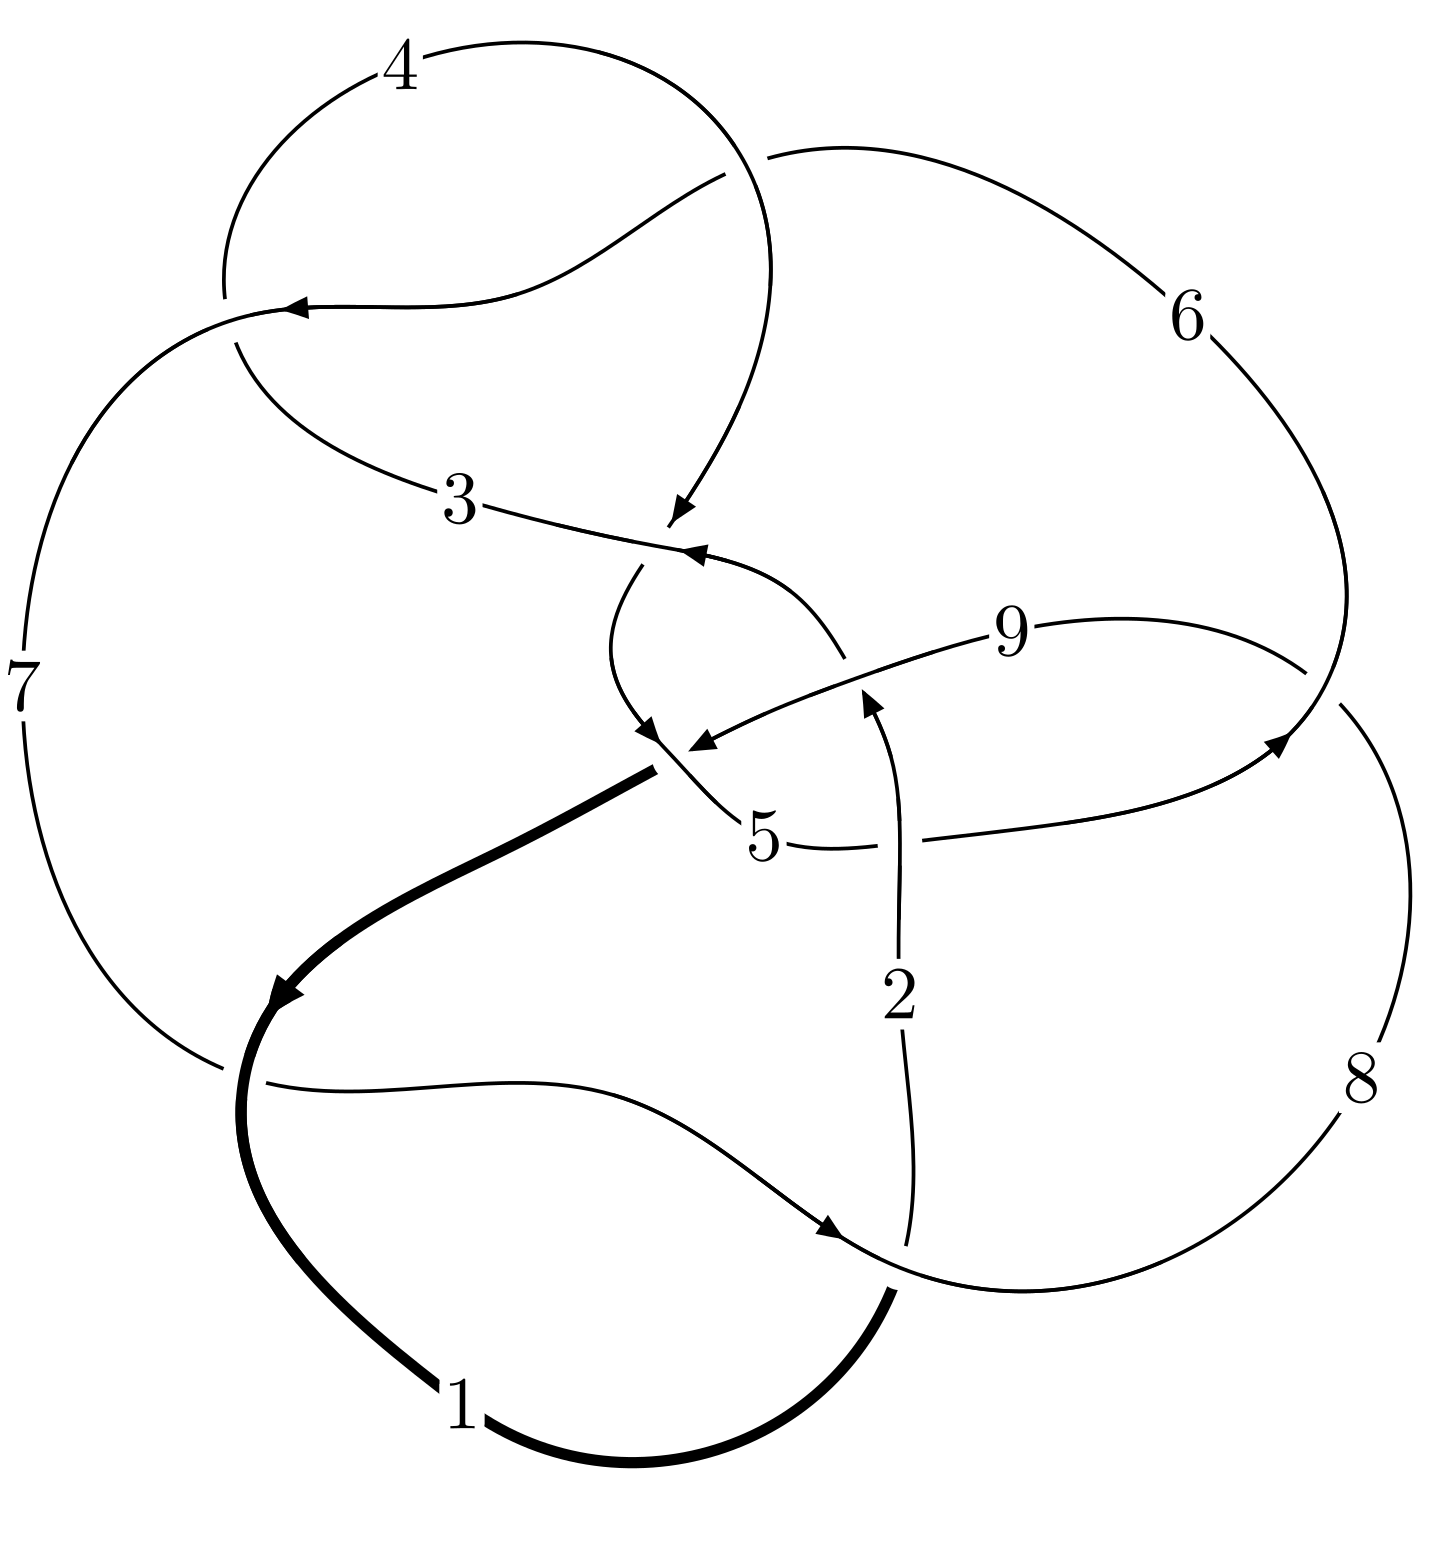
\includegraphics[width=112pt]{../../../GIT/diagram.site/Diagrams/png/68_9_33.png}\\
\ \ \ A knot diagram\footnotemark}&
\allowdisplaybreaks
\textbf{Linearized knot diagam} \\
\cline{2-2}
 &
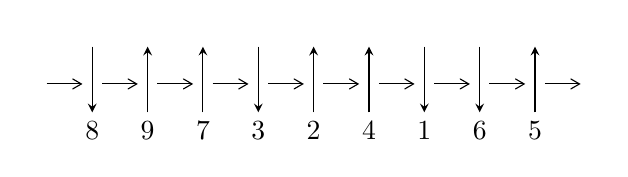
\begin{tikzpicture}[x=20pt, y=17pt]
	% nodes
	\node (C0) at (0, 0) {};
	\node (C1) at (1, 0) {};
	\node (C1U) at (1, +1) {};
	\node (C1D) at (1, -1) {8};

	\node (C2) at (2, 0) {};
	\node (C2U) at (2, +1) {};
	\node (C2D) at (2, -1) {9};

	\node (C3) at (3, 0) {};
	\node (C3U) at (3, +1) {};
	\node (C3D) at (3, -1) {7};

	\node (C4) at (4, 0) {};
	\node (C4U) at (4, +1) {};
	\node (C4D) at (4, -1) {3};

	\node (C5) at (5, 0) {};
	\node (C5U) at (5, +1) {};
	\node (C5D) at (5, -1) {2};

	\node (C6) at (6, 0) {};
	\node (C6U) at (6, +1) {};
	\node (C6D) at (6, -1) {4};

	\node (C7) at (7, 0) {};
	\node (C7U) at (7, +1) {};
	\node (C7D) at (7, -1) {1};

	\node (C8) at (8, 0) {};
	\node (C8U) at (8, +1) {};
	\node (C8D) at (8, -1) {6};

	\node (C9) at (9, 0) {};
	\node (C9U) at (9, +1) {};
	\node (C9D) at (9, -1) {5};
	\node (C10) at (10, 0) {};

	% arrows
	\draw[->,>={angle 60}]
	(C0) edge (C1) (C1) edge (C2) (C2) edge (C3) (C3) edge (C4) (C4) edge (C5) (C5) edge (C6) (C6) edge (C7) (C7) edge (C8) (C8) edge (C9) (C9) edge (C10) ;	\draw[->,>=stealth]
	(C1U) edge (C1D) (C2D) edge (C2U) (C3D) edge (C3U) (C4U) edge (C4D) (C5D) edge (C5U) (C6D) edge (C6U) (C7U) edge (C7D) (C8U) edge (C8D) (C9D) edge (C9U) ;
	\end{tikzpicture} \\
\hhline{~~} \\& 
\textbf{Solving Sequence} \\ \cline{2-2} 
 &
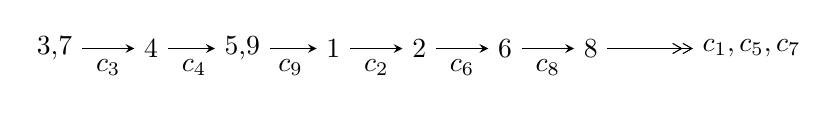
\begin{tikzpicture}[x=31pt, y=7pt]
	% node
	\node (A0) at (-1/8, 0) {3,7};
	\node (A1) at (1, 0) {4};
	\node (A2) at (33/16, 0) {5,9};
	\node (A3) at (25/8, 0) {1};
	\node (A4) at (33/8, 0) {2};
	\node (A5) at (41/8, 0) {6};
	\node (A6) at (49/8, 0) {8};
	\node (C1) at (1/2, -1) {$c_{3}$};
	\node (C2) at (3/2, -1) {$c_{4}$};
	\node (C3) at (21/8, -1) {$c_{9}$};
	\node (C4) at (29/8, -1) {$c_{2}$};
	\node (C5) at (37/8, -1) {$c_{6}$};
	\node (C6) at (45/8, -1) {$c_{8}$};
	\node (A7) at (8, 0) {$c_{1},c_{5},c_{7}$};

	% edge
	\draw[->,>=stealth]	
	(A0) edge (A1) (A1) edge (A2) (A2) edge (A3) (A3) edge (A4) (A4) edge (A5) (A5) edge (A6) ;
	\draw[->>,>={angle 60}]	
	(A6) edge (A7);
\end{tikzpicture} \\ 

\end{tabular} \\

\footnotetext{
The image of knot diagram is generated by the software ``\textbf{Draw programme}" developed by Andrew Bartholomew(\url{http://www.layer8.co.uk/maths/draw/index.htm\#Running-draw}), where we modified some parts for our purpose(\url{https://github.com/CATsTAILs/LinksPainter}).
}\phantom \\ \newline 
\centering \textbf{Ideals for irreducible components\footnotemark of $X_{\text{par}}$} 
 
\begin{align*}
I^u_{1}&=\langle 
523552400 u^{29}-519151600 u^{28}+\cdots+6282411349 b-519170884,\\
\phantom{I^u_{1}}&\phantom{= \langle  }-571526124 u^{29}+47533644 u^{28}+\cdots+6282411349 a+20413019584,\;u^{30}- u^{29}+\cdots-3 u+1\rangle \\
\\
\end{align*}
\raggedright * 1 irreducible components of $\dim_{\mathbb{C}}=0$, with total 30 representations.\\
\footnotetext{All coefficients of polynomials are rational numbers. But the coefficients are sometimes approximated in decimal forms when there is not enough margin.}
\newpage
\renewcommand{\arraystretch}{1}
\centering \section*{I. $I^u_{1}= \langle 5.24\times10^{8} u^{29}-5.19\times10^{8} u^{28}+\cdots+6.28\times10^{9} b-5.19\times10^{8},\;-5.72\times10^{8} u^{29}+4.75\times10^{7} u^{28}+\cdots+6.28\times10^{9} a+2.04\times10^{10},\;u^{30}- u^{29}+\cdots-3 u+1 \rangle$}
\flushleft \textbf{(i) Arc colorings}\\
\begin{tabular}{m{7pt} m{180pt} m{7pt} m{180pt} }
\flushright $a_{3}=$&$\begin{pmatrix}1\\0\end{pmatrix}$ \\
\flushright $a_{7}=$&$\begin{pmatrix}0\\u\end{pmatrix}$ \\
\flushright $a_{4}=$&$\begin{pmatrix}1\\- u^2\end{pmatrix}$ \\
\flushright $a_{5}=$&$\begin{pmatrix}u^2+1\\- u^2\end{pmatrix}$ \\
\flushright $a_{9}=$&$\begin{pmatrix}0.0909724 u^{29}-0.00756615 u^{28}+\cdots+2.67520 u-3.24923\\-0.0833362 u^{29}+0.0826357 u^{28}+\cdots+1.59305 u+0.0826388\end{pmatrix}$ \\
\flushright $a_{1}=$&$\begin{pmatrix}0.816944 u^{29}-0.800274 u^{28}+\cdots+4.33394 u-3.18861\\-0.816587 u^{29}+0.821929 u^{28}+\cdots+1.76785 u+0.0219457\end{pmatrix}$ \\
\flushright $a_{2}=$&$\begin{pmatrix}-0.830556 u^{29}-0.00273693 u^{28}+\cdots-3.66064 u+0.113929\\0.833293 u^{29}-0.830507 u^{28}+\cdots+2.37774 u-0.830556\end{pmatrix}$ \\
\flushright $a_{6}=$&$\begin{pmatrix}- u\\u^3+u\end{pmatrix}$ \\
\flushright $a_{8}=$&$\begin{pmatrix}0.732222 u^{29}-0.798905 u^{28}+\cdots+2.66425 u-3.24557\\-0.733373 u^{29}+0.728883 u^{28}+\cdots+2.69552 u-0.0711119\end{pmatrix}$\\ \flushright $a_{8}=$&$\begin{pmatrix}0.732222 u^{29}-0.798905 u^{28}+\cdots+2.66425 u-3.24557\\-0.733373 u^{29}+0.728883 u^{28}+\cdots+2.69552 u-0.0711119\end{pmatrix}$\\&\end{tabular}
\flushleft \textbf{(ii) Obstruction class $= -1$}\\~\\
\flushleft \textbf{(iii) Cusp Shapes $= -\frac{19978037336}{6282411349} u^{29}+\frac{14950008300}{6282411349} u^{28}+\cdots+\frac{24593576724}{6282411349} u-\frac{28775538078}{6282411349}$}\\~\\
\newpage\renewcommand{\arraystretch}{1}
\flushleft \textbf{(iv) u-Polynomials at the component}\newline \\
\begin{tabular}{m{50pt}|m{274pt}}
Crossings & \hspace{64pt}u-Polynomials at each crossing \\
\hline $$\begin{aligned}c_{1},c_{7}\end{aligned}$$&$\begin{aligned}
&u^{30}- u^{29}+\cdots-5 u+1
\end{aligned}$\\
\hline $$\begin{aligned}c_{2}\end{aligned}$$&$\begin{aligned}
&u^{30}+5 u^{29}+\cdots+u+1
\end{aligned}$\\
\hline $$\begin{aligned}c_{3},c_{6}\end{aligned}$$&$\begin{aligned}
&u^{30}+u^{29}+\cdots+3 u+1
\end{aligned}$\\
\hline $$\begin{aligned}c_{4}\end{aligned}$$&$\begin{aligned}
&u^{30}+13 u^{29}+\cdots+3 u+1
\end{aligned}$\\
\hline $$\begin{aligned}c_{5}\end{aligned}$$&$\begin{aligned}
&u^{30}+3 u^{29}+\cdots+u+1
\end{aligned}$\\
\hline $$\begin{aligned}c_{8}\end{aligned}$$&$\begin{aligned}
&u^{30}-3 u^{29}+\cdots-9 u+1
\end{aligned}$\\
\hline $$\begin{aligned}c_{9}\end{aligned}$$&$\begin{aligned}
&u^{30}- u^{29}+\cdots+11 u+1
\end{aligned}$\\
\hline
\end{tabular}\\~\\
\newpage\renewcommand{\arraystretch}{1}
\flushleft \textbf{(v) Riley Polynomials at the component}\newline \\
\begin{tabular}{m{50pt}|m{274pt}}
Crossings & \hspace{64pt}Riley Polynomials at each crossing \\
\hline $$\begin{aligned}c_{1},c_{7}\end{aligned}$$&$\begin{aligned}
&y^{30}-19 y^{29}+\cdots-5 y+1
\end{aligned}$\\
\hline $$\begin{aligned}c_{2}\end{aligned}$$&$\begin{aligned}
&y^{30}-3 y^{29}+\cdots-5 y+1
\end{aligned}$\\
\hline $$\begin{aligned}c_{3},c_{6}\end{aligned}$$&$\begin{aligned}
&y^{30}+13 y^{29}+\cdots+3 y+1
\end{aligned}$\\
\hline $$\begin{aligned}c_{4}\end{aligned}$$&$\begin{aligned}
&y^{30}+9 y^{29}+\cdots+39 y+1
\end{aligned}$\\
\hline $$\begin{aligned}c_{5}\end{aligned}$$&$\begin{aligned}
&y^{30}+5 y^{29}+\cdots+3 y+1
\end{aligned}$\\
\hline $$\begin{aligned}c_{8}\end{aligned}$$&$\begin{aligned}
&y^{30}-27 y^{29}+\cdots+11 y+1
\end{aligned}$\\
\hline $$\begin{aligned}c_{9}\end{aligned}$$&$\begin{aligned}
&y^{30}-23 y^{29}+\cdots-9 y+1
\end{aligned}$\\
\hline
\end{tabular}\\~\\
\newpage\flushleft \textbf{(vi) Complex Volumes and Cusp Shapes}
$$\begin{array}{c|c|c}  
\text{Solutions to }I^u_{1}& \I (\text{vol} + \sqrt{-1}CS) & \text{Cusp shape}\\
 \hline 
\begin{aligned}
u &= \phantom{-}0.907923 + 0.426568 I \\
a &= -1.169900 + 0.764529 I \\
b &= \phantom{-}1.065260 - 0.854723 I\end{aligned}
 & -0.60287 - 7.55963 I & \phantom{-}1.09191 + 4.94493 I \\ \hline\begin{aligned}
u &= \phantom{-}0.907923 - 0.426568 I \\
a &= -1.169900 - 0.764529 I \\
b &= \phantom{-}1.065260 + 0.854723 I\end{aligned}
 & -0.60287 + 7.55963 I & \phantom{-}1.09191 - 4.94493 I \\ \hline\begin{aligned}
u &= \phantom{-}0.365761 + 0.979876 I \\
a &= -1.59795 + 1.33270 I \\
b &= \phantom{-}1.43354 + 0.57946 I\end{aligned}
 & -4.52085 + 1.19841 I & -7.97414 - 1.50646 I \\ \hline\begin{aligned}
u &= \phantom{-}0.365761 - 0.979876 I \\
a &= -1.59795 - 1.33270 I \\
b &= \phantom{-}1.43354 - 0.57946 I\end{aligned}
 & -4.52085 - 1.19841 I & -7.97414 + 1.50646 I \\ \hline\begin{aligned}
u &= -0.485323 + 0.928263 I \\
a &= \phantom{-}1.61933 - 1.81589 I \\
b &= -0.365965 - 0.331561 I\end{aligned}
 & -1.86283 - 2.41995 I & \phantom{-}7.1505 - 13.4441 I \\ \hline\begin{aligned}
u &= -0.485323 - 0.928263 I \\
a &= \phantom{-}1.61933 + 1.81589 I \\
b &= -0.365965 + 0.331561 I\end{aligned}
 & -1.86283 + 2.41995 I & \phantom{-}7.1505 + 13.4441 I \\ \hline\begin{aligned}
u &= \phantom{-}0.702308 + 0.543288 I \\
a &= \phantom{-}1.12249 - 1.09131 I \\
b &= -1.170130 + 0.757580 I\end{aligned}
 & \phantom{-}2.66519 - 2.12888 I & \phantom{-}4.79788 + 2.27450 I \\ \hline\begin{aligned}
u &= \phantom{-}0.702308 - 0.543288 I \\
a &= \phantom{-}1.12249 + 1.09131 I \\
b &= -1.170130 - 0.757580 I\end{aligned}
 & \phantom{-}2.66519 + 2.12888 I & \phantom{-}4.79788 - 2.27450 I \\ \hline\begin{aligned}
u &= -0.630570 + 0.920314 I \\
a &= -1.078230 - 0.484581 I \\
b &= \phantom{-}0.527369 - 0.255959 I\end{aligned}
 & \phantom{-}0.59733 - 2.56045 I & \phantom{-}2.74559 + 1.69203 I \\ \hline\begin{aligned}
u &= -0.630570 - 0.920314 I \\
a &= -1.078230 + 0.484581 I \\
b &= \phantom{-}0.527369 + 0.255959 I\end{aligned}
 & \phantom{-}0.59733 + 2.56045 I & \phantom{-}2.74559 - 1.69203 I\\
 \hline 
 \end{array}$$\newpage$$\begin{array}{c|c|c}  
\text{Solutions to }I^u_{1}& \I (\text{vol} + \sqrt{-1}CS) & \text{Cusp shape}\\
 \hline 
\begin{aligned}
u &= -0.419790 + 0.765608 I \\
a &= -0.38715 + 1.97907 I \\
b &= -0.071716 + 0.565767 I\end{aligned}
 & -1.28380 - 1.43143 I & -4.72992 + 7.90920 I \\ \hline\begin{aligned}
u &= -0.419790 - 0.765608 I \\
a &= -0.38715 - 1.97907 I \\
b &= -0.071716 - 0.565767 I\end{aligned}
 & -1.28380 + 1.43143 I & -4.72992 - 7.90920 I \\ \hline\begin{aligned}
u &= \phantom{-}0.488147 + 1.019990 I \\
a &= \phantom{-}0.469424 + 0.779563 I \\
b &= \phantom{-}0.91649 - 1.42667 I\end{aligned}
 & -3.68107 + 4.90989 I & -5.62064 - 7.63658 I \\ \hline\begin{aligned}
u &= \phantom{-}0.488147 - 1.019990 I \\
a &= \phantom{-}0.469424 - 0.779563 I \\
b &= \phantom{-}0.91649 + 1.42667 I\end{aligned}
 & -3.68107 - 4.90989 I & -5.62064 + 7.63658 I \\ \hline\begin{aligned}
u &= -0.874083 + 0.729953 I \\
a &= -0.810701 - 0.043239 I \\
b &= \phantom{-}0.692011 - 0.163163 I\end{aligned}
 & \phantom{-}0.99971 - 3.02182 I & \phantom{-}5.70717 + 7.15965 I \\ \hline\begin{aligned}
u &= -0.874083 - 0.729953 I \\
a &= -0.810701 + 0.043239 I \\
b &= \phantom{-}0.692011 + 0.163163 I\end{aligned}
 & \phantom{-}0.99971 + 3.02182 I & \phantom{-}5.70717 - 7.15965 I \\ \hline\begin{aligned}
u &= \phantom{-}0.104954 + 0.846587 I \\
a &= -1.013570 + 0.508000 I \\
b &= -0.214087 + 1.056250 I\end{aligned}
 & -1.84656 - 1.46172 I & -3.40911 + 4.12645 I \\ \hline\begin{aligned}
u &= \phantom{-}0.104954 - 0.846587 I \\
a &= -1.013570 - 0.508000 I \\
b &= -0.214087 - 1.056250 I\end{aligned}
 & -1.84656 + 1.46172 I & -3.40911 - 4.12645 I \\ \hline\begin{aligned}
u &= \phantom{-}0.606261 + 1.034690 I \\
a &= \phantom{-}1.77136 - 0.83961 I \\
b &= -1.26265 - 1.09290 I\end{aligned}
 & \phantom{-}1.20556 + 7.17470 I & \phantom{-}1.40394 - 7.73482 I \\ \hline\begin{aligned}
u &= \phantom{-}0.606261 - 1.034690 I \\
a &= \phantom{-}1.77136 + 0.83961 I \\
b &= -1.26265 + 1.09290 I\end{aligned}
 & \phantom{-}1.20556 - 7.17470 I & \phantom{-}1.40394 + 7.73482 I\\
 \hline 
 \end{array}$$\newpage$$\begin{array}{c|c|c}  
\text{Solutions to }I^u_{1}& \I (\text{vol} + \sqrt{-1}CS) & \text{Cusp shape}\\
 \hline 
\begin{aligned}
u &= -0.739608 + 0.193899 I \\
a &= \phantom{-}0.491712 - 0.140537 I \\
b &= -0.711939 + 0.029552 I\end{aligned}
 & \phantom{-}1.50909 - 0.09583 I & \phantom{-}7.75398 - 0.81660 I \\ \hline\begin{aligned}
u &= -0.739608 - 0.193899 I \\
a &= \phantom{-}0.491712 + 0.140537 I \\
b &= -0.711939 - 0.029552 I\end{aligned}
 & \phantom{-}1.50909 + 0.09583 I & \phantom{-}7.75398 + 0.81660 I \\ \hline\begin{aligned}
u &= \phantom{-}0.066161 + 1.287720 I \\
a &= \phantom{-}0.153531 - 0.197790 I \\
b &= \phantom{-}0.644560 - 0.905239 I\end{aligned}
 & -6.75726 - 4.69908 I & -5.55546 + 4.95856 I \\ \hline\begin{aligned}
u &= \phantom{-}0.066161 - 1.287720 I \\
a &= \phantom{-}0.153531 + 0.197790 I \\
b &= \phantom{-}0.644560 + 0.905239 I\end{aligned}
 & -6.75726 + 4.69908 I & -5.55546 - 4.95856 I \\ \hline\begin{aligned}
u &= \phantom{-}0.651249 + 1.142680 I \\
a &= -1.59583 + 0.80518 I \\
b &= \phantom{-}1.15164 + 1.02775 I\end{aligned}
 & -2.77714 + 13.28050 I & -1.34939 - 8.37714 I \\ \hline\begin{aligned}
u &= \phantom{-}0.651249 - 1.142680 I \\
a &= -1.59583 - 0.80518 I \\
b &= \phantom{-}1.15164 - 1.02775 I\end{aligned}
 & -2.77714 - 13.28050 I & -1.34939 + 8.37714 I \\ \hline\begin{aligned}
u &= -0.611458 + 1.208770 I \\
a &= \phantom{-}0.528417 + 0.484423 I \\
b &= -0.632962 + 0.456161 I\end{aligned}
 & -1.48004 - 5.18678 I & -0.12994 + 9.32507 I \\ \hline\begin{aligned}
u &= -0.611458 - 1.208770 I \\
a &= \phantom{-}0.528417 - 0.484423 I \\
b &= -0.632962 - 0.456161 I\end{aligned}
 & -1.48004 + 5.18678 I & -0.12994 - 9.32507 I \\ \hline\begin{aligned}
u &= \phantom{-}0.368067 + 0.266876 I \\
a &= -2.50293 - 0.01848 I \\
b &= \phantom{-}0.498568 + 0.860476 I\end{aligned}
 & -1.90369 - 1.10699 I & -1.88237 + 2.02123 I \\ \hline\begin{aligned}
u &= \phantom{-}0.368067 - 0.266876 I \\
a &= -2.50293 + 0.01848 I \\
b &= \phantom{-}0.498568 - 0.860476 I\end{aligned}
 & -1.90369 + 1.10699 I & -1.88237 - 2.02123 I\\
 \hline 
 \end{array}$$\newpage
\newpage\renewcommand{\arraystretch}{1}
\centering \section*{ II. u-Polynomials}
\begin{tabular}{m{50pt}|m{274pt}}
Crossings & \hspace{64pt}u-Polynomials at each crossing \\
\hline $$\begin{aligned}c_{1},c_{7}\end{aligned}$$&$\begin{aligned}
&u^{30}- u^{29}+\cdots-5 u+1
\end{aligned}$\\
\hline $$\begin{aligned}c_{2}\end{aligned}$$&$\begin{aligned}
&u^{30}+5 u^{29}+\cdots+u+1
\end{aligned}$\\
\hline $$\begin{aligned}c_{3},c_{6}\end{aligned}$$&$\begin{aligned}
&u^{30}+u^{29}+\cdots+3 u+1
\end{aligned}$\\
\hline $$\begin{aligned}c_{4}\end{aligned}$$&$\begin{aligned}
&u^{30}+13 u^{29}+\cdots+3 u+1
\end{aligned}$\\
\hline $$\begin{aligned}c_{5}\end{aligned}$$&$\begin{aligned}
&u^{30}+3 u^{29}+\cdots+u+1
\end{aligned}$\\
\hline $$\begin{aligned}c_{8}\end{aligned}$$&$\begin{aligned}
&u^{30}-3 u^{29}+\cdots-9 u+1
\end{aligned}$\\
\hline $$\begin{aligned}c_{9}\end{aligned}$$&$\begin{aligned}
&u^{30}- u^{29}+\cdots+11 u+1
\end{aligned}$\\
\hline
\end{tabular}\newpage\renewcommand{\arraystretch}{1}
\centering \section*{ III. Riley Polynomials}
\begin{tabular}{m{50pt}|m{274pt}}
Crossings & \hspace{64pt}Riley Polynomials at each crossing \\
\hline $$\begin{aligned}c_{1},c_{7}\end{aligned}$$&$\begin{aligned}
&y^{30}-19 y^{29}+\cdots-5 y+1
\end{aligned}$\\
\hline $$\begin{aligned}c_{2}\end{aligned}$$&$\begin{aligned}
&y^{30}-3 y^{29}+\cdots-5 y+1
\end{aligned}$\\
\hline $$\begin{aligned}c_{3},c_{6}\end{aligned}$$&$\begin{aligned}
&y^{30}+13 y^{29}+\cdots+3 y+1
\end{aligned}$\\
\hline $$\begin{aligned}c_{4}\end{aligned}$$&$\begin{aligned}
&y^{30}+9 y^{29}+\cdots+39 y+1
\end{aligned}$\\
\hline $$\begin{aligned}c_{5}\end{aligned}$$&$\begin{aligned}
&y^{30}+5 y^{29}+\cdots+3 y+1
\end{aligned}$\\
\hline $$\begin{aligned}c_{8}\end{aligned}$$&$\begin{aligned}
&y^{30}-27 y^{29}+\cdots+11 y+1
\end{aligned}$\\
\hline $$\begin{aligned}c_{9}\end{aligned}$$&$\begin{aligned}
&y^{30}-23 y^{29}+\cdots-9 y+1
\end{aligned}$\\
\hline
\end{tabular}
\vskip 2pc
\end{document}